\begin{figure}[ht!]
  \centering
\begin{subfigure}{1.0\linewidth}
\centering
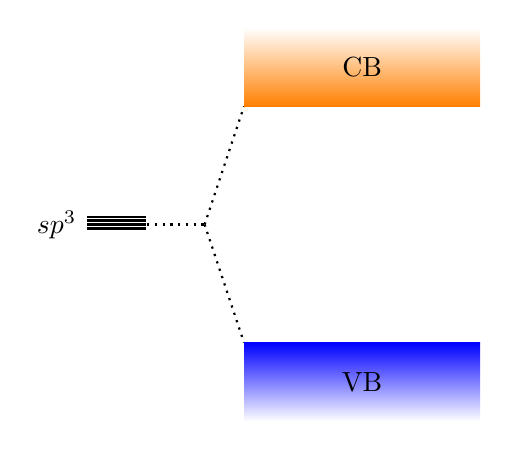
\begin{tikzpicture}

  \atom[name=C, color=orange, pos={(-2,0)},scale=0.5]{
    gray/45/45/0,
    gray/315/315/0,
    gray/225/225/0,
    gray/135/135/0}

  \draw[thick,-] (-1.25,-4) -- (-2.0,-4) node[anchor=east]{$sp^3$};
  \draw[thick,-] (-1.25,-3.95) -- (-2.0,-3.95);
  \draw[thick,-] (-1.25,-4.05) -- (-2.0,-4.05);
  \draw[thick,-] (-1.25,-3.90) -- (-2.0,-3.90);

  \draw[thick, dotted] (-1.23,-4) -- (-0.5,-4);
  \draw[thick, dotted] (-0.5,-4) -- (0,-5.5);
  \draw[thick, dotted] (-0.5,-4) -- (0,-2.5);

  %\node at (1.5,1.5) {$E_g$};
  %\draw (0,-1.5) -- (2,-1.5) -- (2,-2) -- (0,-2) -- (0,0);
  \shade[top color=white,bottom color=orange] (0,-2.5) rectangle (3.0,-1.5) node[pos=.5] {CB};
  \shade[top color=blue,bottom color=white] (0.,-6.5) rectangle (3.0,-5.5) node[pos=.5] {VB};

  \atom[name=C, color=orange, scale=0.5]{
    gray/45/45/0,
    gray/315/315/0,
    gray/225/225/0,
    gray/135/135/0}
  \atom[name=C, color=orange, pos={(0.75,0.75)},scale=0.5]{
    gray/45/45/0,
    gray/315/315/0,
    gray/225/225/0,
    gray/135/135/0}
  \atom[name=C, color=orange, pos={(1.5,0)},scale=0.5]{
    gray/45/45/0,
    gray/315/315/0,
    gray/225/225/0,
    gray/135/135/0}
  \atom[name=C, color=orange, pos={(0.75,-0.75)},scale=0.5]{
    gray/45/45/0,
    gray/315/315/0,
    gray/225/225/0,
    gray/135/135/0}
  \atom[name=C, color=orange, pos={(2.25,0.75)},scale=0.5]{
    gray/45/45/0,
    gray/315/315/0,
    gray/225/225/0,
    gray/135/135/0}
  \atom[name=C, color=orange, pos={(2.25,-0.75)},scale=0.5]{
    gray/45/45/0,
    gray/315/315/0,
    gray/225/225/0,
    gray/135/135/0}
  \atom[name=C, color=orange, pos={(3.0,0)},scale=0.5]{
      gray/45/45/0,
      gray/315/315/0,
      gray/225/225/0,
      gray/135/135/0}

\end{tikzpicture}
\subcaption{} \label{fig:diamond structure}
\end{subfigure}%

\begin{subfigure}{1.0\linewidth}
\centering
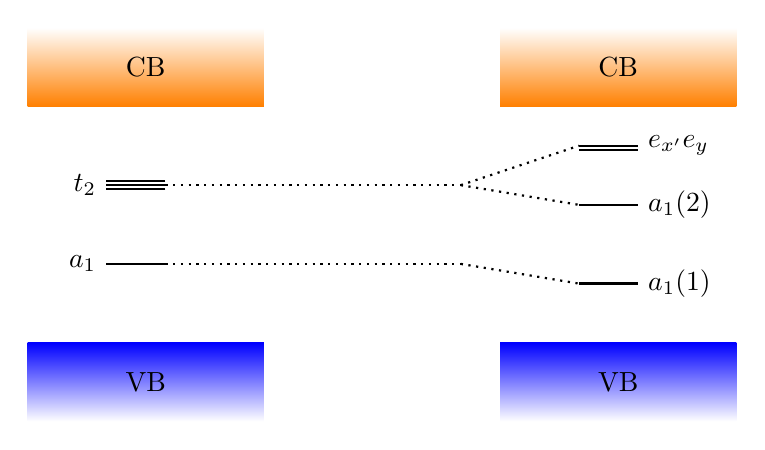
\begin{tikzpicture}

  \shade[top color=white,bottom color=orange] (0.-7,-2.5) rectangle (3.0-7,-1.5) node[pos=.5] {CB};
  \shade[top color=blue,bottom color=white] (0.-7,-6.5) rectangle (3.0-7,-5.5) node[pos=.5] {VB};

  \draw[thick,-] (1.75-7,-4.5) -- (1.0-7,-4.5) node[anchor=east]{$a_1$};
  \draw[thick,-] (1.75-7,-3.5) -- (1.0-7,-3.5) node[anchor=east]{$t_2$};
  \draw[thick,-] (1.75-7,-3.55) -- (1.0-7,-3.55);
  \draw[thick,-] (1.75-7,-3.45) -- (1.0-7,-3.45);

  \atom[name=C, color=orange, pos={(0-7,0)}, scale=0.5]{
    gray/45/45/0,
    gray/315/315/0,
    gray/225/225/0,
    gray/135/135/0}
  \atom[name=C, color=orange, pos={(0.75-7,0.75)},scale=0.5]{
    gray/45/45/0,
    red/315/315/0,
    gray/225/225/0,
    gray/135/135/0}
  \atom[name=v, color=gray, pos={(1.5-7,0)},scale=0.5]{}
  \atom[name=C, color=orange, pos={(0.75-7,-0.75)},scale=0.5]{
    red/45/45/0,
    gray/315/315/0,
    gray/225/225/0,
    gray/135/135/0}
  \atom[name=C, color=orange, pos={(2.25-7,0.75)},scale=0.5]{
    gray/45/45/0,
    gray/315/315/0,
    red/225/225/0,
    gray/135/135/0}
  \atom[name=C, color=orange, pos={(2.25-7,-0.75)},scale=0.5]{
    gray/45/45/0,
    gray/315/315/0,
    gray/225/225/0,
    red/135/135/0}
  \atom[name=C, color=orange, pos={(3.0-7,0)},scale=0.5]{
      gray/45/45/0,
      gray/315/315/0,
      gray/225/225/0,
      gray/135/135/0}

    \shade[top color=white,bottom color=orange] (0.-1.,-2.5) rectangle (3.0-1.0,-1.5) node[pos=.5] {CB};
    \shade[top color=blue,bottom color=white] (0.-1.,-6.5) rectangle (3.0-1.0,-5.5) node[pos=.5] {VB};

    \atom[name=C, color=orange, pos={(0.-1.,0)}, scale=0.5]{
      gray/45/45/0,
      blue/315/315/0,
      gray/225/225/0,
      gray/135/135/0}
    \atom[name=C, color=orange, pos={(0.75-1,0.75)},scale=0.5]{
      gray/45/45/0,
      red/315/315/0,
      gray/225/225/0,
      gray/135/135/0}
    \atom[name=v, color=gray, pos={(1.5-1,0)},scale=0.5]{}
    \atom[name=N, color=green!95, pos={(0.75-1,-0.75)},scale=0.5]{
      blue/45/45/0,
      blue/315/315/0,
      blue/225/225/0,
      blue/135/135/0}
    \atom[name=C, color=orange, pos={(2.25-1,0.75)},scale=0.5]{
      gray/45/45/0,
      gray/315/315/0,
      red/225/225/0,
      gray/135/135/0}
    \atom[name=C, color=orange, pos={(2.25-1,-0.75)},scale=0.5]{
      gray/45/45/0,
      gray/315/315/0,
      gray/225/225/0,
      red/135/135/0}
    \atom[name=C, color=orange, pos={(3.0-1,0)},scale=0.5]{
        gray/45/45/0,
        gray/315/315/0,
        gray/225/225/0,
        gray/135/135/0}

    \draw[thick, dotted] (1.75-7,-3.5) -- (-1.5,-3.5);
    \draw[thick, dotted] (-1.5,-3.5) -- (0,-3.0);
    \draw[thick, dotted] (-1.5,-3.5) -- (0,-3.75);

    \draw[thick,-] (1.0-1,-3.0) -- (1.75-1,-3.0) node[anchor=west]{$e_{x'}e_y$};
        \draw[thick,-] (1.75-1,-3.05) -- (1.0-1,-3.05);
    \draw[thick,-] (1.0-1,-3.75) -- (1.75-1,-3.75) node[anchor=west]{$a_1(2)$};

    \draw[thick, dotted] (1.75-7,-4.5) -- (-1.5,-4.5);
    \draw[thick, dotted] (-1.5,-4.5) -- (0,-4.75);
    \draw[thick,-] (1.0-1,-4.75) -- (1.75-1,-4.75) node[anchor=west]{$a_1(1)$};

\end{tikzpicture}
\subcaption{} \label{fig:defect diamond structure}
\end{subfigure}
\par\bigskip
\caption{A schematic representation of the electronic structure of the NV$^{-1}$ defect in a tetrahedrally coordinated semiconductor, exemplified by diamond. Figure used from Ref. \cite{Gordon2013}.}
\label{fig: diamond electronic structure}
\end{figure}
